\chapter{System Design}
This project was written entirely within Unity so in this section I will be dealing with the structure of the Unity game and I will go into how different aspects of the game work with explanations and references to relevant snippets of code or algorithms used.
\section{Scenes}
For SlimeWorld there are two scenes, the main menu which the player enters upon starting the application and the game scene in which the simulation occurs. The main menu contains, buttons to enter the main game, to quit the game and also to open the settings menu where the parameters of the simulation can be altered using a set of sliders.
\section{Menu Scene}
The menu scene is the simpler of the two scenes and it is responsible for giving the users the opportunity to change the settings of the simulation and to launch the simulation.  This image \ref{image:mainMenuHierarchy} shows the hierarchy of the scene in the Unity editor. As seen here there are two sets of menus, the "main" menu and the settings menu.
\begin{figure}[ht!]
    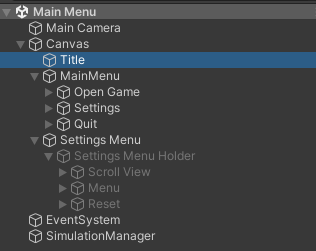
\includegraphics[width=0.5\textwidth]{images/MainMenuHierarchy.png}
    \caption{Main Menu Hierarchy}
    \label{image:mainMenuHierarchy}
\end{figure}

\subsubsection{Main Menu}
The main menu as seen here \ref{image:mainMenuPicture} is very simple containing the title of the game at the top of the screen and 3 buttons: Play, Settings and Quit. The play button sends the player into the Game scene, the Settings button opens the settings menu and the Quit button causes the game to close.
\begin{figure}[ht!]
    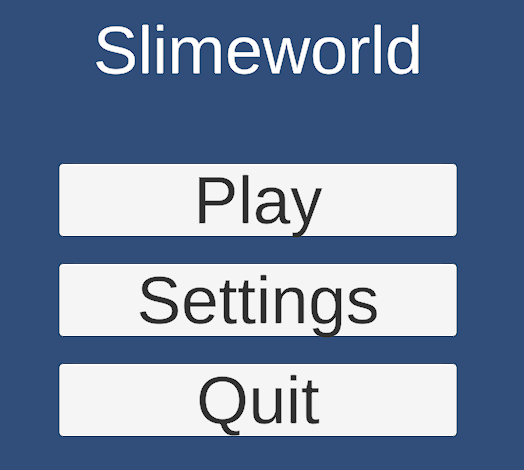
\includegraphics[width=0.5\textwidth]{images/MainMenuPicture.png}
    \caption{Picture of the Main Menu}
    \label{image:mainMenuPicture}
\end{figure}
\subsubsection{Settings Menu}
The settings menu as seen here \ref{image:settingsPicture} contains a scrollable view which contains the settings for the different parameters of the simulation, which are altered using the sliders. When the settings menu is opened, the SettingsMenu script gets all of the settings properties which are associated with the SimulationManager script and assigns them to the relevant sliders. When a slider is used, it calls the relevant method attached to slider, passing in its updated value and the updated value is in turn assigned to the relevant property of the SimulationManager and saved as a player preference. If the user clicks Menu the settings menu will be deactivated and the main menu will be reactivated. If the user clicks Reset, all playerprefs will be wiped, resetting settings to default values and also returning the player to the main menu.
\begin{figure}[ht!]
    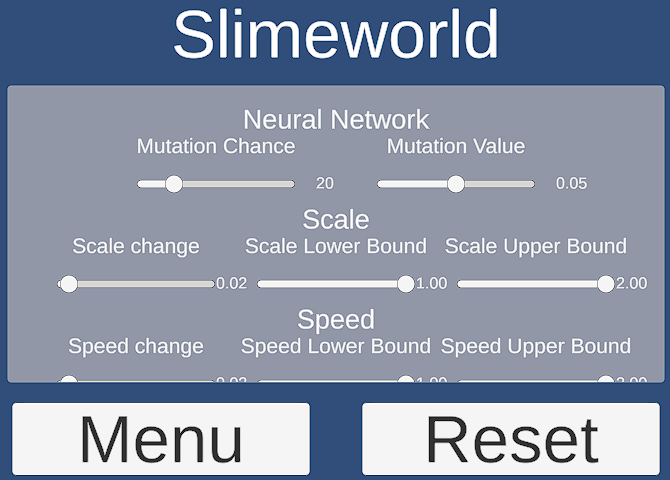
\includegraphics[width=0.5\textwidth]{images/SettingsPicture.png}
    \caption{Picture of the Settings Menu}
    \label{image:settingsPicture}
\end{figure}
\subsubsection{Simulation Manager}
The Simulation Manager is a singleton script which is shared across both the Menu and Game scenes, but I shall put it in the Menu scene as in normal usage of the application, the menu scene is where it is initialized. The SimulationManager script is responsible for loading and storing saved user settings and handling any modifications of the properties used to store them.
\par
The SimulationManager makes use of the singleton design principle to enable easier inter-script communication as access to its properties is required by many of the scripts in the game scene, including the SlimeManager script, FoodManager script and NeuralNetwork script.
\par
The SimulationManager makes heavy use of C\# properties to handle manipulation of settings and an example of one such property is found in this code snippet \ref{lst:cSharpProperty}. Where the properties of the property make it easy and convenient to handle modification of \_mutationChance variable and make it easy to determine when a property is modified.
\begin{lstlisting}[language=csh, caption=C\# Property, label={lst:cSharpProperty}]
    private int _mutationChance;
    public int MutationChance
    {
        get => _mutationChance;
        set
        {
            _mutationChance = value;
            PlayerPrefs.SetInt("MutationChance", value);
        }
    }
\end{lstlisting}
\section{Game Scene}
The Game scene is the main scene of the game and is responsible for the simulation of evolution by providing a small environment in which the slime can spawn and eat and reproduce or die. This image \ref{image:gameHierarchy} shows the hierarcy of the scene in the Unity editor.
\begin{figure}[ht!]
    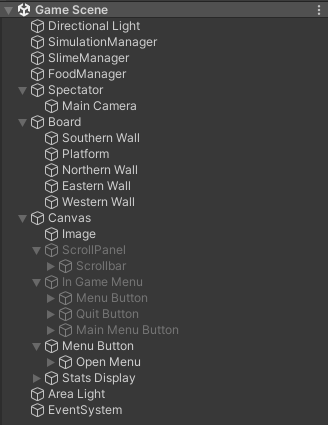
\includegraphics[width=0.5\textwidth]{images/GameSceneHierarchy.png}
    \caption{Game Hierarchy}
    \label{image:gameHierarchy}
\end{figure}
\subsection{Slime Manager}
The SlimeManager is a singleton script which is responsible for the spawning and disabling of slimes, upon entering the game scene or if the number of slimes dips too low, the SlimeManager will trigger a method called SpawnWave, which will spawn a number of slimes decided by the setting in the settings menu mentioned earlier.
\par
The SlimeManager is responsible for the spawning of slimes both with and without parent slimes, and to this end, the SlimeManager contains an instance of ObjectPool which stores slime GameObjects. When the SlimeManager spawns a slime it first must calculate the position of the new slime, which is a random position anywhere on the board if the slime is parent-less and is within 2 units on the x and the y axis of the parent if the slime has a parent. The SlimeManager then gets an instance of the slime GameObject from ObjectPool, assigns it a name which is Slime\_ followed by a number representing the number of slimes that had spawned before it. 
\par
For slimes without parents, the scale and speed values are determined randomly with regard to the lower and upper bounds for each value determined using the settings menu, a code snippet explaining this alongside the names is here \ref{lst:parentlessSlime}. 

\begin{lstlisting}[language=csh, caption=Parent-less Slime, label={lst:parentlessSlime}]
    spawnedSlime.name = string.Format("Slime_{0:00000}", _slimeCount++);
        Slime spawnedSlimeScript = spawnedSlime.GetComponent<Slime>();

        //float scale = UnityEngine.Random.Range(0.5f, 2f);
        //float speed = UnityEngine.Random.Range(0.5f, 2f);

        float scale = UnityEngine.Random.Range(SimulationManager.Instance().ScaleLowerBound, SimulationManager.Instance().ScaleUpperBound);
        float speed = UnityEngine.Random.Range(SimulationManager.Instance().SpeedLowerBound, SimulationManager.Instance().SpeedUpperBound);

        // pseudo constructor method for game object
        spawnedSlimeScript.Init(scale, speed);
\end{lstlisting}
\par
For slimes with parents, the method is much more complicated and takes the parent slime as a parameter. Seen here is the code \ref{lst:parentedSlime}, some of which has been removed for conciseness, but as can be seen, the child slime takes the parent's generation plus 1, receives a copy of their slimeInfo and a copy of their neural network.
\begin{lstlisting}[language=csh, caption=Slime with Parent, label={lst:parentedSlime}]
        // generation = parents generation + 1
        int generation = parentSlimeScript.GetGeneration() + 1;

        // parent's slime info is saved to be passed in to save variable
        SlimeInfo slimeInfo = parentSlimeScript.GetSlimeInfo();

        // parent's neural network is saved to be passed in
        NeuralNetwork neuralNetwork = parentSlimeScript.GetNeuralNetwork();

        // As it is unwise to create instance of classes extending monobehaviours using the new command, the init command is used as a pseudo constructor after the gameobject has been instantiated
        spawnedSlimeScript.Init(scale, speed, generation, slimeInfo, neuralNetwork);
\end{lstlisting}
\par
The last responsibility of the SlimeManager as mentioned earlier is to deactivate slimes when they've either been eaten or rotted away and to this, the SlimeManager simply calls the DeactivateObject method on the slime in question, returning it to the object pool.
\subsection{Slime}
The Slime is the most important class in the scene and game, as it represents the creatures which are being evolved in the simulation. The slimes have a number of persistent variables associated with them, their scale and speed which are floats, their generation which is an int, alongside their slimeInfo which is a SlimeInfo and their neuralNetwork which is a NeuralNetwork. All of these are inherited from a parent if said parent exists.
\par
The slime's scale represents its size and if a slime is 10\% larger than a smaller slime, it can eat the slime upon collision and convert it to saturation, which is a measure of the number of calories the slime has. The slime's speed represents its movement speed. Both scale and speed have a metabolic cost in the simulation with slimes with higher numbers in either trait having a proportionally higher energy upkeep.
\par
The SlimeInfo is a simple class used to store a slime's name, scale, speed, generation and number of children alongside the instance of its parent SlimeInfo, this is used to create a sort of linked-list of slimeInfos which can be used to keep track of the ancestry of slimes. Here is a code snippet \ref{lst:parentedSlimeInfo}, which contains the constructor for SlimeInfo when a slime has a parent.
\begin{lstlisting}[language=csh, caption=Slime Info with Parent, label={lst:parentedSlimeInfo}]
        // Constructor for slime with parent, takes the generation and parentSlime as additional paramters
    public SlimeInfo(string slimeName, float slimeSize, float slimeSpeed, int slimeGeneration, SlimeInfo parentSlime)
    {
        SlimeName = slimeName;
        SlimeScale = slimeSize;
        SlimeSpeed = slimeSpeed;
        SlimeGeneration = slimeGeneration;
        // The SlimeInfo parentSlime is a way to set the connect the parentSlimeInfo to this slimeInfo approximating a linked list
        ParentSlime = parentSlime;
        SlimeChildren = 0;
    }
\end{lstlisting}
\par
The slimes behaviours are controlled by a neural network which is a mutated copy of their parent's neural network, though the mechanics of this will be analyzed more in-depth in the Neural Network section.
\subsection{Neural Network}
The Neural Network implemented in SlimeWorld is a simple neural network which does not make any use of back-propagation or other more advanced training techniques, the reason for this is that in order to more accurately approximate evolution, the neural network has no scoring parameters for evaluating its performance, and with the sandbox nature of the simulation it would be rather awkward to try and set any parameters by which to measure the success of the neural network. 
\par
To this end, the neural network is one of the simplest variants, with the modifications being an unmodified random chance, which is applied equally to every weight and bias in the network. The downsides of this approach are obvious in that the neural network will neither be trained quickly nor to a high degree of accuracy.

\subsubsection{Inputs and Outputs}
For the neural network, one decision I made early on was that I wanted to ensure that every input was normalized to be within the same range, this was a design decision that I could implement without too much difficulty as all inputs would be generated by the slimes in-game. As I had settled on tanh as my activation function, I decided to keep all inputs and outputs of the neural network between -1 and 1.
\par
The topology of the neural network that I have used for this project is 12 nodes in the inputs layer, 8 nodes in the first hidden layer, 5 nodes in the second hidden layer, and 2 output nodes. I have classified the input nodes into three sections based on what kind of information they contribute to the neural network, the first being internal information \ref{lst:neuralNetworkThisSlime}, being information that pertains to the slime itself and contains 3 input nodes.
\begin{lstlisting}[language=csh, caption=Neural Networks inputs for The Slime, label={lst:neuralNetworkThisSlime}]
    // Represents slimes current hunger, updates every in-game update
    _inputsToNeural[0] = _saturation / 50f - 1f;

    // Setting neural inputs that persist for the life of the slime, as neither _scale nor _speed can change, these inputs are set once and never changed
    _inputsToNeural[1] = _scale;
    _inputsToNeural[2] = _speed;
\end{lstlisting}
\par
The next category of information for the slime is that related to food which contains 3 input nodes \ref{lst:neuralNetworkFood}. and the final category of information being that related to other slimes which contain 6 input nodes \ref{lst:neuralNetworkOtherSlimes}.
\begin{lstlisting}[language=csh, caption=Neural Networks inputs for Food, label={lst:neuralNetworkFood}]
     // Represents saturation of food, -0.5f due to following formula
    // value = (saturation / 50) - 1, so for food which has default 25 = -0.5f
    _inputsToNeural[3] = -0.5f;
    // Represents angle of food relative to slime in pi radians to fit in with scheme of inputs being -1 to 1,
    // Negative values are on the left side, positive values are on the right
    _inputsToNeural[4] = (Mathf.Deg2Rad * Vector2.Angle(transform.forward, (Vector2)(_closestFood.transform.position - transform.position))) - 1;
    // Represents distance to food from slime, with values between -1 and 1,
    // And distance greater than 25 is capped at an input value of 1
    _inputsToNeural[5] = Mathf.Clamp((Vector3.Distance(_closestFood.transform.position, transform.position) / 12.5f) - 1f, -1f, 1f);
\end{lstlisting}
\begin{lstlisting}[language=csh, caption=Neural Networks inputs for other slime, label={lst:neuralNetworkOtherSlimes}]
    Slime closestSlimeScript =
    _closestSlime.GetComponent<Slime>();
    // Represents scale of closestSlime, values are clamped between 0.5 and 2 typically
    // So take away one to fit within established scheme for neural net inputs
    _inputsToNeural[6] = closestSlimeScript.GetScale() - 1;
    // Represents speed of closestSlime, values are clamped between 0.5 and 2 typically
    // So take away one to fit within established scheme for neural net inputs
    _inputsToNeural[7] = closestSlimeScript.GetSpeed() - 1;
    // Represents angle of closestSlime relative to slime in pi radians to fit in with scheme of inputs being -1 to 1,
    // Negative values are on the left side, positive values are on the right
    _inputsToNeural[8] = (Mathf.Deg2Rad * Vector2.Angle(transform.forward, (Vector2)(_closestSlime.transform.position - transform.position))) - 1;
    // Represents distance to closestSlime from slime, with values between -1 and 1,
    // And distance greater than 25 is capped at an input value of 1
    _inputsToNeural[9] = Mathf.Clamp((Vector3.Distance(_closestFood.transform.position, transform.position) / 12.5f) - 1f, -1f, 1f);
    // Represents saturation value of closestSlime, calculated with following formula,
    // input = (saturationIfEaten / 50) = 1
    _inputsToNeural[10] = (closestSlimeScript.GetSaturationIfEaten() / 50f) - 1;
    // Represents status of closestSlime, 0 if dead, 1 if alive
    _inputsToNeural[11] = closestSlimeScript.IsAlive() ? 1 : 0;
\end{lstlisting}
\par
The training of the neural network is performed with a very naive and inefficient method, where when a NetworkNetwork is cloned from another, each bias and weight has a chance of changing a given amount based on the input parameters, which are set in the settings menu mentioned earlier.
\subsection{Food Manager}
The FoodManager script is a singleton responsible for the creation and removal of food in the simulation. The FoodManager has an ObjectPool instance containing a prefab for a food GameObject. Upon starting the game and every 10 seconds thereafter a specified amount of food, determined by the foodPerInterval setting is spawned unless the foodCap is reached at which point no more food will spawn until the food dips below the cap. When food is spawned, a food GameObject is pulled from the objectPool and placed at a random location on the map. And when a piece of food is eaten, it calls the FoodManager's DeactivateFood method which in turn calls the ObjectPool's DeactivateObject method.
\subsection{Object Pool}
I created my own implementation of an object pool as I felt that the object pool incorporated in Unity didn't properly satisfy my requirements. One of the key reasons was that I desired the ability to keep track of all active objects in the pool so that I could more easily perform checks to determine which entities were closest to one another by iterating through every entity on the list of active objects.
\par
The object pool is composed of list of GameObjects containing the active objects in game and a queue of GameObjects representing all the deactivated objects in the game. I picked a list to represent the active objects as I wished to be able to iterate through the list easily, while I felt that a queue would suit the inactive objects better, as all that was necessary was to store objects that were deactivated and then pop them from the front of the queue once a new object was needed.
\par
To make use of the object pool, I created a constructor which would take in the gameObject representing the prefab to be stored as a parameter as can be seen in this listing \ref{lst:ObjectPool}. I then made use of the object pools to store prefabs of both the foods and the slimes as both are frequently created and destroyed in the simulation.
\begin{lstlisting}[language=csh, caption=Object pool, label={lst:ObjectPool}]
    public ObjectPool(GameObject pooledObject)
    {
        _activeObjectPool = new List<GameObject>();
        _inactiveObjectPool = new Queue<GameObject>();
        _pooledObject = pooledObject;
    }
\end{lstlisting}
\par
After making the object pool, I had to make methods to use the object pool to provide objects when necessary which can be seen in this code snippet \ref{lst:ObjectPoolActivateDeactivate}. The purpose of the DeactivateObject method was to take in objects that were to be deactivated, set them to inactive, remove them from the list of active objects and then add them to the queue of inactive objects. The GetPooledObject method would check if the queue of inactive objects was empty and if so it would instantiate a new object based on the stored prefab, otherwise it would pop the deactivated object at the head of the queue and activate it, before returning it.
\begin{lstlisting}[language=csh, caption = Object pool activate and deactivate, label={lst:ObjectPoolActivateDeactivate}]
// Passed in object is deactivated, removed from the activepool and added to inactivepool
    public void DeactivateObject(GameObject objectToDeactivate)
    {
        objectToDeactivate.SetActive(false);
        _activeObjectPool.Remove(objectToDeactivate);
        _inactiveObjectPool.Enqueue(objectToDeactivate);
    }

    // Either returns an object from the inactiveObjectPool or instantiates a new object if the inactiveObjectPool is empty
    public GameObject GetPooledObject()
    {
        // Object variable is declared
        GameObject objectToReturn;
        if (_inactiveObjectPool.Count != 0)
        {
            // if inactivePool isn't empty then take object from queue
            objectToReturn = _inactiveObjectPool.Dequeue();
            objectToReturn.SetActive(true);
        }
        else
        {
            // if pool is empty then instatiate new object
            objectToReturn = Object.Instantiate(_pooledObject);
        }
        // object is added to activeObjectPool
        _activeObjectPool.Add(objectToReturn);
        return objectToReturn;
    }
\end{lstlisting}
\section{Spectator}
The spectator represents the user's camera and is a flying object which is controlled using WASD, E and Q for movement forwards, left, back and right and up and down. The Spectator uses the mouse for rotation, though if the escape is pressed, the cursor is unlocked so that it can interface with the UI. If the left mouse button is clicked while the user is moused over a slime, the statistics relevant to the slime and their ancestry is displayed \ref{image:inGameUI}.
\begin{figure}[ht!]
    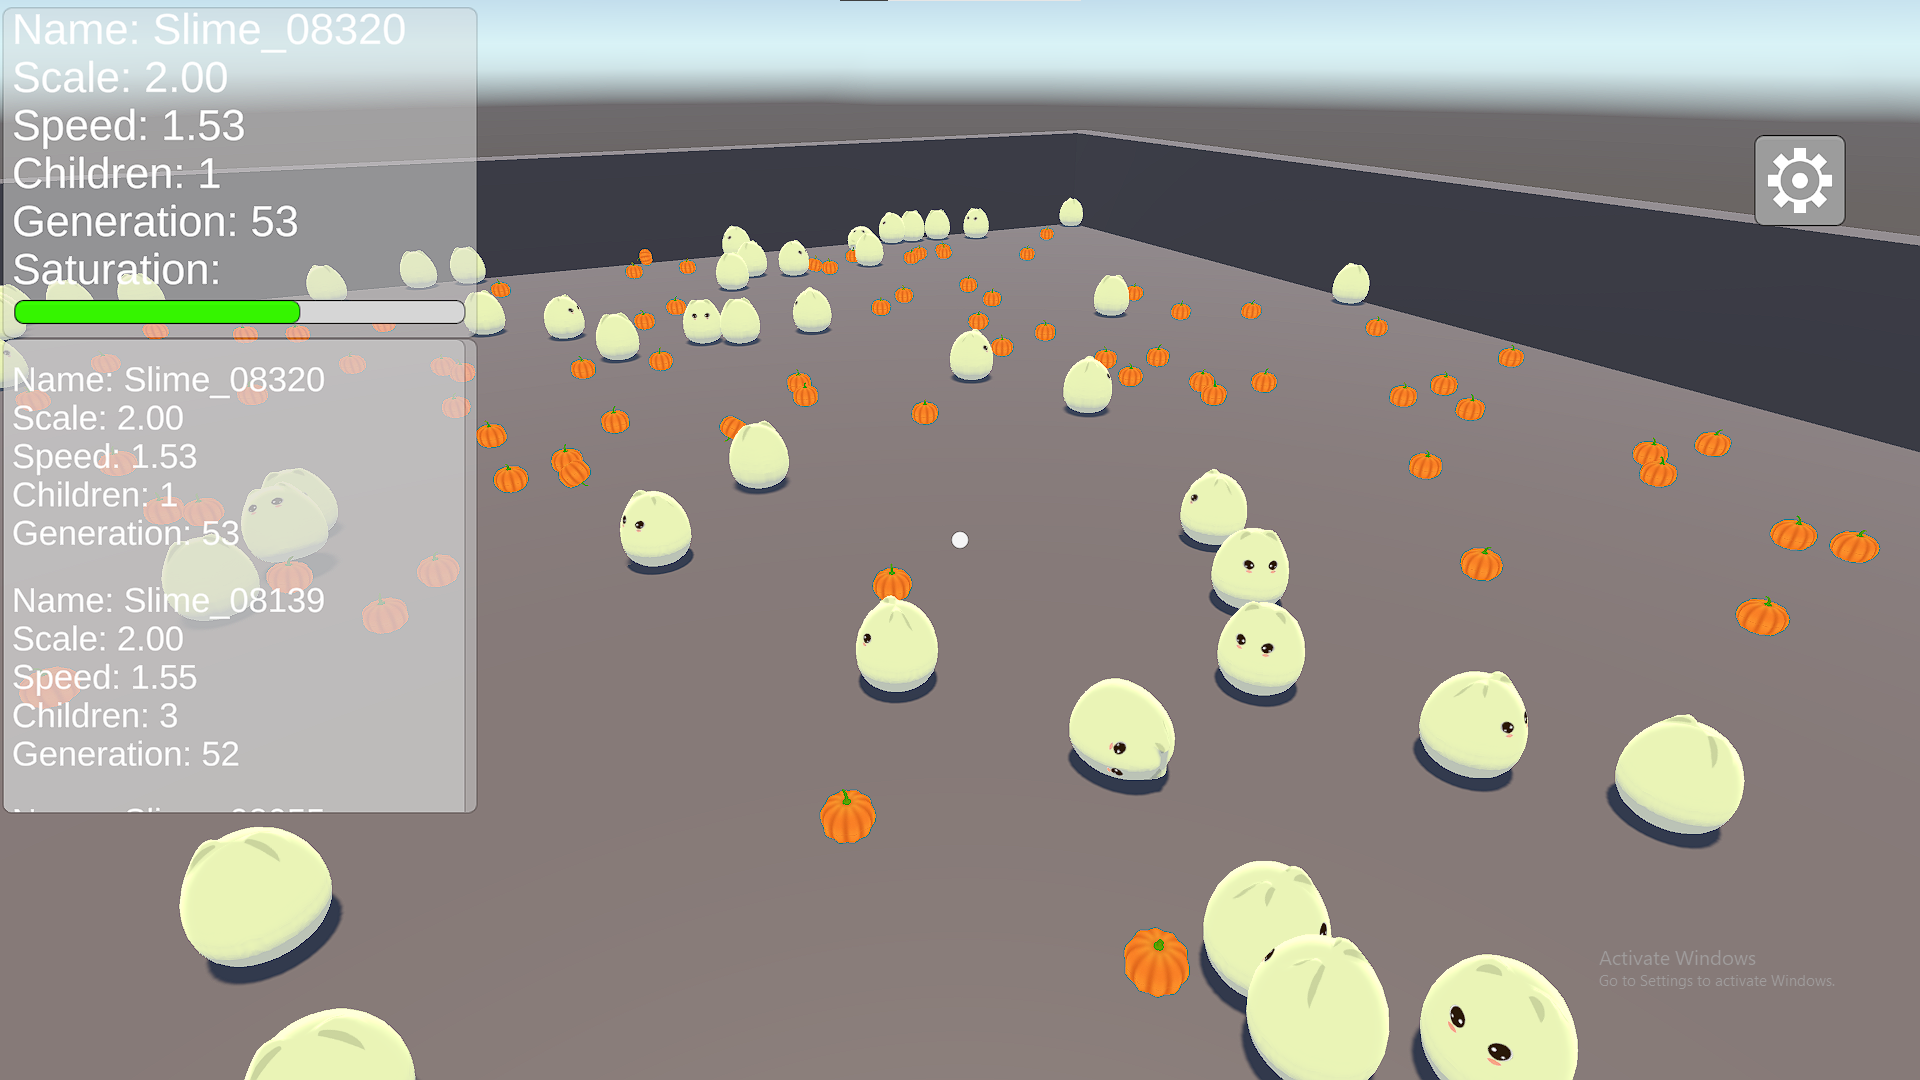
\includegraphics[width=0.5\textwidth]{images/GameUI.png}
    \caption{In-Game UI}
    \label{image:inGameUI}
\end{figure}
\par
The ancestry data, being populated using the slime's slimeInfo, and the attached reference to the previous generation's slime info, to iterate through them all and generate a list. Which is then assigned to a scroll-able list on the left side of the screen.
\par
if the user's mouse is unlocked and they click on the gear on the right side of the screen they open the in-game menu from which they have buttons to return to the main menu, quit the game outright or close the in-game menu \ref{image:inGameMenu}.
\begin{figure}[ht!]
    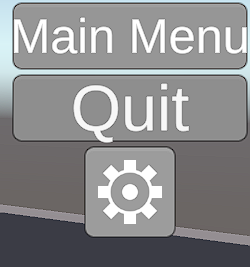
\includegraphics[width=0.5\textwidth]{images/Game Menu.png}
    \caption{In-Game Menu}
    \label{image:inGameMenu}
\end{figure}